% Options for packages loaded elsewhere
\PassOptionsToPackage{unicode}{hyperref}
\PassOptionsToPackage{hyphens}{url}
%
\documentclass[
]{book}
\usepackage{amsmath,amssymb}
\usepackage{iftex}
\ifPDFTeX
  \usepackage[T1]{fontenc}
  \usepackage[utf8]{inputenc}
  \usepackage{textcomp} % provide euro and other symbols
\else % if luatex or xetex
  \usepackage{unicode-math} % this also loads fontspec
  \defaultfontfeatures{Scale=MatchLowercase}
  \defaultfontfeatures[\rmfamily]{Ligatures=TeX,Scale=1}
\fi
\usepackage{lmodern}
\ifPDFTeX\else
  % xetex/luatex font selection
\fi
% Use upquote if available, for straight quotes in verbatim environments
\IfFileExists{upquote.sty}{\usepackage{upquote}}{}
\IfFileExists{microtype.sty}{% use microtype if available
  \usepackage[]{microtype}
  \UseMicrotypeSet[protrusion]{basicmath} % disable protrusion for tt fonts
}{}
\makeatletter
\@ifundefined{KOMAClassName}{% if non-KOMA class
  \IfFileExists{parskip.sty}{%
    \usepackage{parskip}
  }{% else
    \setlength{\parindent}{0pt}
    \setlength{\parskip}{6pt plus 2pt minus 1pt}}
}{% if KOMA class
  \KOMAoptions{parskip=half}}
\makeatother
\usepackage{xcolor}
\usepackage{color}
\usepackage{fancyvrb}
\newcommand{\VerbBar}{|}
\newcommand{\VERB}{\Verb[commandchars=\\\{\}]}
\DefineVerbatimEnvironment{Highlighting}{Verbatim}{commandchars=\\\{\}}
% Add ',fontsize=\small' for more characters per line
\usepackage{framed}
\definecolor{shadecolor}{RGB}{248,248,248}
\newenvironment{Shaded}{\begin{snugshade}}{\end{snugshade}}
\newcommand{\AlertTok}[1]{\textcolor[rgb]{0.94,0.16,0.16}{#1}}
\newcommand{\AnnotationTok}[1]{\textcolor[rgb]{0.56,0.35,0.01}{\textbf{\textit{#1}}}}
\newcommand{\AttributeTok}[1]{\textcolor[rgb]{0.13,0.29,0.53}{#1}}
\newcommand{\BaseNTok}[1]{\textcolor[rgb]{0.00,0.00,0.81}{#1}}
\newcommand{\BuiltInTok}[1]{#1}
\newcommand{\CharTok}[1]{\textcolor[rgb]{0.31,0.60,0.02}{#1}}
\newcommand{\CommentTok}[1]{\textcolor[rgb]{0.56,0.35,0.01}{\textit{#1}}}
\newcommand{\CommentVarTok}[1]{\textcolor[rgb]{0.56,0.35,0.01}{\textbf{\textit{#1}}}}
\newcommand{\ConstantTok}[1]{\textcolor[rgb]{0.56,0.35,0.01}{#1}}
\newcommand{\ControlFlowTok}[1]{\textcolor[rgb]{0.13,0.29,0.53}{\textbf{#1}}}
\newcommand{\DataTypeTok}[1]{\textcolor[rgb]{0.13,0.29,0.53}{#1}}
\newcommand{\DecValTok}[1]{\textcolor[rgb]{0.00,0.00,0.81}{#1}}
\newcommand{\DocumentationTok}[1]{\textcolor[rgb]{0.56,0.35,0.01}{\textbf{\textit{#1}}}}
\newcommand{\ErrorTok}[1]{\textcolor[rgb]{0.64,0.00,0.00}{\textbf{#1}}}
\newcommand{\ExtensionTok}[1]{#1}
\newcommand{\FloatTok}[1]{\textcolor[rgb]{0.00,0.00,0.81}{#1}}
\newcommand{\FunctionTok}[1]{\textcolor[rgb]{0.13,0.29,0.53}{\textbf{#1}}}
\newcommand{\ImportTok}[1]{#1}
\newcommand{\InformationTok}[1]{\textcolor[rgb]{0.56,0.35,0.01}{\textbf{\textit{#1}}}}
\newcommand{\KeywordTok}[1]{\textcolor[rgb]{0.13,0.29,0.53}{\textbf{#1}}}
\newcommand{\NormalTok}[1]{#1}
\newcommand{\OperatorTok}[1]{\textcolor[rgb]{0.81,0.36,0.00}{\textbf{#1}}}
\newcommand{\OtherTok}[1]{\textcolor[rgb]{0.56,0.35,0.01}{#1}}
\newcommand{\PreprocessorTok}[1]{\textcolor[rgb]{0.56,0.35,0.01}{\textit{#1}}}
\newcommand{\RegionMarkerTok}[1]{#1}
\newcommand{\SpecialCharTok}[1]{\textcolor[rgb]{0.81,0.36,0.00}{\textbf{#1}}}
\newcommand{\SpecialStringTok}[1]{\textcolor[rgb]{0.31,0.60,0.02}{#1}}
\newcommand{\StringTok}[1]{\textcolor[rgb]{0.31,0.60,0.02}{#1}}
\newcommand{\VariableTok}[1]{\textcolor[rgb]{0.00,0.00,0.00}{#1}}
\newcommand{\VerbatimStringTok}[1]{\textcolor[rgb]{0.31,0.60,0.02}{#1}}
\newcommand{\WarningTok}[1]{\textcolor[rgb]{0.56,0.35,0.01}{\textbf{\textit{#1}}}}
\usepackage{longtable,booktabs,array}
\usepackage{calc} % for calculating minipage widths
% Correct order of tables after \paragraph or \subparagraph
\usepackage{etoolbox}
\makeatletter
\patchcmd\longtable{\par}{\if@noskipsec\mbox{}\fi\par}{}{}
\makeatother
% Allow footnotes in longtable head/foot
\IfFileExists{footnotehyper.sty}{\usepackage{footnotehyper}}{\usepackage{footnote}}
\makesavenoteenv{longtable}
\usepackage{graphicx}
\makeatletter
\def\maxwidth{\ifdim\Gin@nat@width>\linewidth\linewidth\else\Gin@nat@width\fi}
\def\maxheight{\ifdim\Gin@nat@height>\textheight\textheight\else\Gin@nat@height\fi}
\makeatother
% Scale images if necessary, so that they will not overflow the page
% margins by default, and it is still possible to overwrite the defaults
% using explicit options in \includegraphics[width, height, ...]{}
\setkeys{Gin}{width=\maxwidth,height=\maxheight,keepaspectratio}
% Set default figure placement to htbp
\makeatletter
\def\fps@figure{htbp}
\makeatother
\setlength{\emergencystretch}{3em} % prevent overfull lines
\providecommand{\tightlist}{%
  \setlength{\itemsep}{0pt}\setlength{\parskip}{0pt}}
\setcounter{secnumdepth}{5}
\usepackage{booktabs}
\usepackage{ctex}
\usepackage[a4paper, margin=1in]{geometry}
\setlength{\parindent}{2em}
\ifLuaTeX
  \usepackage{selnolig}  % disable illegal ligatures
\fi
\usepackage[]{natbib}
\bibliographystyle{plainnat}
\IfFileExists{bookmark.sty}{\usepackage{bookmark}}{\usepackage{hyperref}}
\IfFileExists{xurl.sty}{\usepackage{xurl}}{} % add URL line breaks if available
\urlstyle{same}
\hypersetup{
  pdftitle={R语言与精算数据科学},
  pdfauthor={张连增 李浩男},
  hidelinks,
  pdfcreator={LaTeX via pandoc}}

\title{R语言与精算数据科学}
\author{张连增 \quad 李浩男}
\date{2024-09-02}

\begin{document}
\maketitle

{
\setcounter{tocdepth}{1}
\tableofcontents
}
\chapter{前言}\label{ux524dux8a00}

R语言是一种专门用于统计分析和数据可视化的编程语言和软件环境。它由统计学家Ross Ihaka和Robert Gentleman于1993年开发,并且是基于S语言的一种实现。R语言在学术界、统计学界、数据科学以及相关领域中被广泛使用。

\section{为什么选择R?}\label{ux4e3aux4ec0ux4e48ux9009ux62e9r}

\begin{enumerate}
\def\labelenumi{\arabic{enumi}.}
\item
  \textbf{强大的统计功能}: R语言内置了丰富的统计分析功能,支持回归分析、假设检验、时间序列分析、聚类分析等多种统计方法,且不断有新的包和函数被开发和维护。
\item
  \textbf{数据可视化}:R语言提供了强大的数据可视化功能,尤其是通过\texttt{ggplot2}包可以创建高度定制化和复杂的图表。R语言支持的图表种类非常多样,包括散点图、柱状图、箱线图、热图等。
\item
  \textbf{开放性与扩展性}:R是一个开源项目,拥有庞大的用户和开发者社区。CRAN(Comprehensive R Archive Network)上有数千个扩展包,覆盖了几乎所有的数据分析需求,从生物信息学到金融分析。
\item
  \textbf{与其他语言和工具的兼容性}:R可以与其他编程语言(如Python、C++)以及数据管理工具(如SQL、Hadoop)集成,这使得它能够处理大型数据集,并与其他数据处理工作流无缝衔接。
\item
  \textbf{交互性和易用性}:R语言有丰富的交互式环境(如RStudio),用户可以方便地编写、调试代码,并实时查看分析结果。此外,R语言的语法相对直观,适合统计学背景的用户。
\item
  \textbf{广泛的应用领域}:R在金融、医药、生物信息学、社会科学等多个领域都有广泛应用。它被用于学术研究、数据科学项目以及商业分析中。
\end{enumerate}

\section{精算与R语言}\label{ux7cbeux7b97ux4e0erux8bedux8a00}

精算学是一个集数学、统计学、经济学、金融学及计算机科学于一体的综合性学科,它专注于对金融风险和不确定性进行量化评估,为保险、养老金、投资等行业提供决策支持。而R语言作为一种强大的统计分析和图形展示工具,在精算领域的应用日益广泛,以下是几个主要原因:

\begin{itemize}
\item
  \begin{enumerate}
  \def\labelenumi{\arabic{enumi}.}
  \tightlist
  \item
    数据分析和建模:精算师需要处理大量数据,包括保险赔付记录、客户资料、市场趋势等。R语言提供了丰富的统计和数据分析包(如\texttt{ggplot2}用于数据可视化,\texttt{dplyr}和\texttt{tidyr}用于数据清洗和整理,\texttt{lm}、\texttt{glm}等函数用于线性模型和非线性模型拟合),能够高效地帮助精算师进行数据清洗、探索性数据分析、模型构建和验证等步骤。
  \end{enumerate}
\item
  \begin{enumerate}
  \def\labelenumi{\arabic{enumi}.}
  \setcounter{enumi}{1}
  \tightlist
  \item
    风险管理和预测:精算的核心工作之一是评估未来风险并制定相应的保险费率、准备金等。R语言能够支持各种复杂的预测模型,如时间序列分析(\texttt{forecast}包)、生存分析(\texttt{survival}包)以及机器学习算法(通过\texttt{caret}、\texttt{randomForest}等包),这些工具对于预测保险损失、评估长寿风险等至关重要。
  \end{enumerate}
\item
  \begin{enumerate}
  \def\labelenumi{\arabic{enumi}.}
  \setcounter{enumi}{2}
  \tightlist
  \item
    报告和可视化:精算师需要向管理层、监管机构或客户报告分析结果。R语言不仅能处理复杂的数据分析,还能生成高质量的图形和报告,通过R Markdown、Shiny等工具,可以轻松地创建交互式报告和仪表板,使数据分析和结果呈现更加直观和易于理解。
  \end{enumerate}
\item
  \begin{enumerate}
  \def\labelenumi{\arabic{enumi}.}
  \setcounter{enumi}{3}
  \tightlist
  \item
    行业趋势和前沿技术:随着大数据和人工智能的发展,精算行业也在不断探索新技术的应用。R语言作为开源社区活跃的统计软件,不断吸收和整合新的算法和技术,如深度学习、自然语言处理等,为精算师提供了接触和应用前沿技术的平台。
  \end{enumerate}
\item
  \begin{enumerate}
  \def\labelenumi{\arabic{enumi}.}
  \setcounter{enumi}{4}
  \tightlist
  \item
    就业竞争力:掌握R语言将极大地提升精算专业学生的就业竞争力。在保险、金融等行业,具备数据分析能力的人才越来越受到重视。能够熟练运用R语言进行数据分析、模型构建和报告呈现的学生,在求职过程中将更具优势。
  \end{enumerate}
\end{itemize}

在CRAN网站中包含了专门针对精算学的R语言项目集合,参考\url{https://cran.r-project.org/web/views/ActuarialScience.html}。其中提供了一系列R包,覆盖了寿险精算中的生存分析、死亡率模型;非寿险计算中的损失模型、产品定价、准备金计算;再保险与极值理论;精算相关的数据集等内容。

\chapter{你好, R!}\label{ux4f60ux597d-r}

\section{R 软件: 安装 R 和 RStudio}\label{r-ux8f6fux4ef6-ux5b89ux88c5-r-ux548c-rstudio}

R 可以从以下网站下载: \url{http://cran.r-project.org/}。
R可用于所有平台: Unix/Linux、Windows 和 Mac。在本课程中,我们还将使用 RStudio,一个 R 的界面。RStudio 可以从 \url{www.rstudio.org} 获取。RStudio 可作为桌面程序用于所有平台: Unix/Linux、Windows 和 Mac。
在本教程中,我们将重点关注 R 的 Windows 实现。

\section{R GUI软件交互界面}\label{r-guiux8f6fux4ef6ux4ea4ux4e92ux754cux9762}

\begin{figure}

{\centering 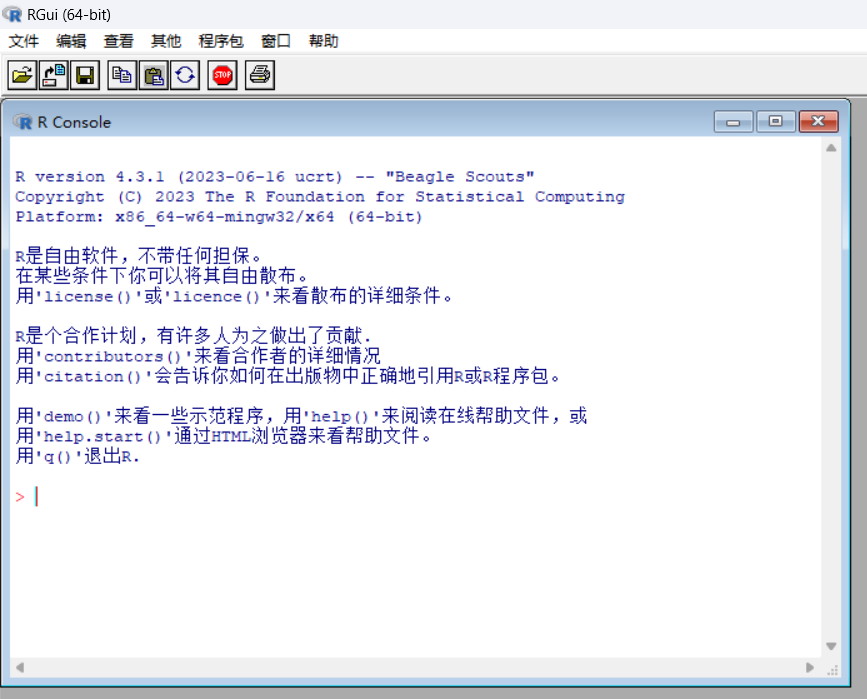
\includegraphics[width=0.8\linewidth]{figs/01-Rinterface} 

}

\caption{R软件启动界面}\label{fig:Rgui}
\end{figure}

当我们启动 R Studio 软件后,可以看到提示符 \(>\),这个提示符现在正在等待你的命令,如图\ref{fig:Rgui}。下面我们可以用一行命令实现一系列高级操作,生成了若干张图片。

\begin{Shaded}
\begin{Highlighting}[]
\FunctionTok{demo}\NormalTok{(graphics)}
\end{Highlighting}
\end{Shaded}

这行代码帮助我们完成了\texttt{demo}函数的调用,在R中,调用函数时需要加上括号,括号内是函数的参数,我们会在后续的学习深入了解函数的概念,并实现自编R函数。如果我们要了解更多关于 \texttt{demo} 函数的参数和选项的信息,我们可以查看 \texttt{demo} 的帮助。要获取帮助,只需使用 \texttt{help} 命令或在命令前输入问号 \texttt{?}。感兴趣的话可以试试\texttt{?demo}或\texttt{help(demo)},你会得到更多类似的命令。

\subsection{中断和退出R}\label{ux4e2dux65adux548cux9000ux51far}

如果你希望中断一个正在执行的代码,在 Windows 或 MacOS 上按 \texttt{ESC} 键,或者点击工具栏的``停止标志''(它是红色的)。
如果你希望退出 R,你可以点击窗口框架右上角的红色 X(Windows),按 CMD+q(MacOS)。在所有平台上,你可以输入:

\begin{Shaded}
\begin{Highlighting}[]
\FunctionTok{q}\NormalTok{()}
\end{Highlighting}
\end{Shaded}

在这个界面中,我们可以直接输入代码并得到结果,但是使用起来并不方便,推荐使用RStudio。

\section{RStudio 软件}\label{rstudio-ux8f6fux4ef6}

RStudio 是为 R 语言设计的一个跨平台的集成开发环境(IDE),它将许多功能强大的编程工具集成到一个直观、易于学习的界面中。用户可以在其中编辑、运行 R 的程序文件,可以跟踪运行,还可以构造文字、图表融合在一起的研究报告等。 一个运行中的RStudio界面见图\ref{fig:Rstudio}。

\begin{figure}

{\centering 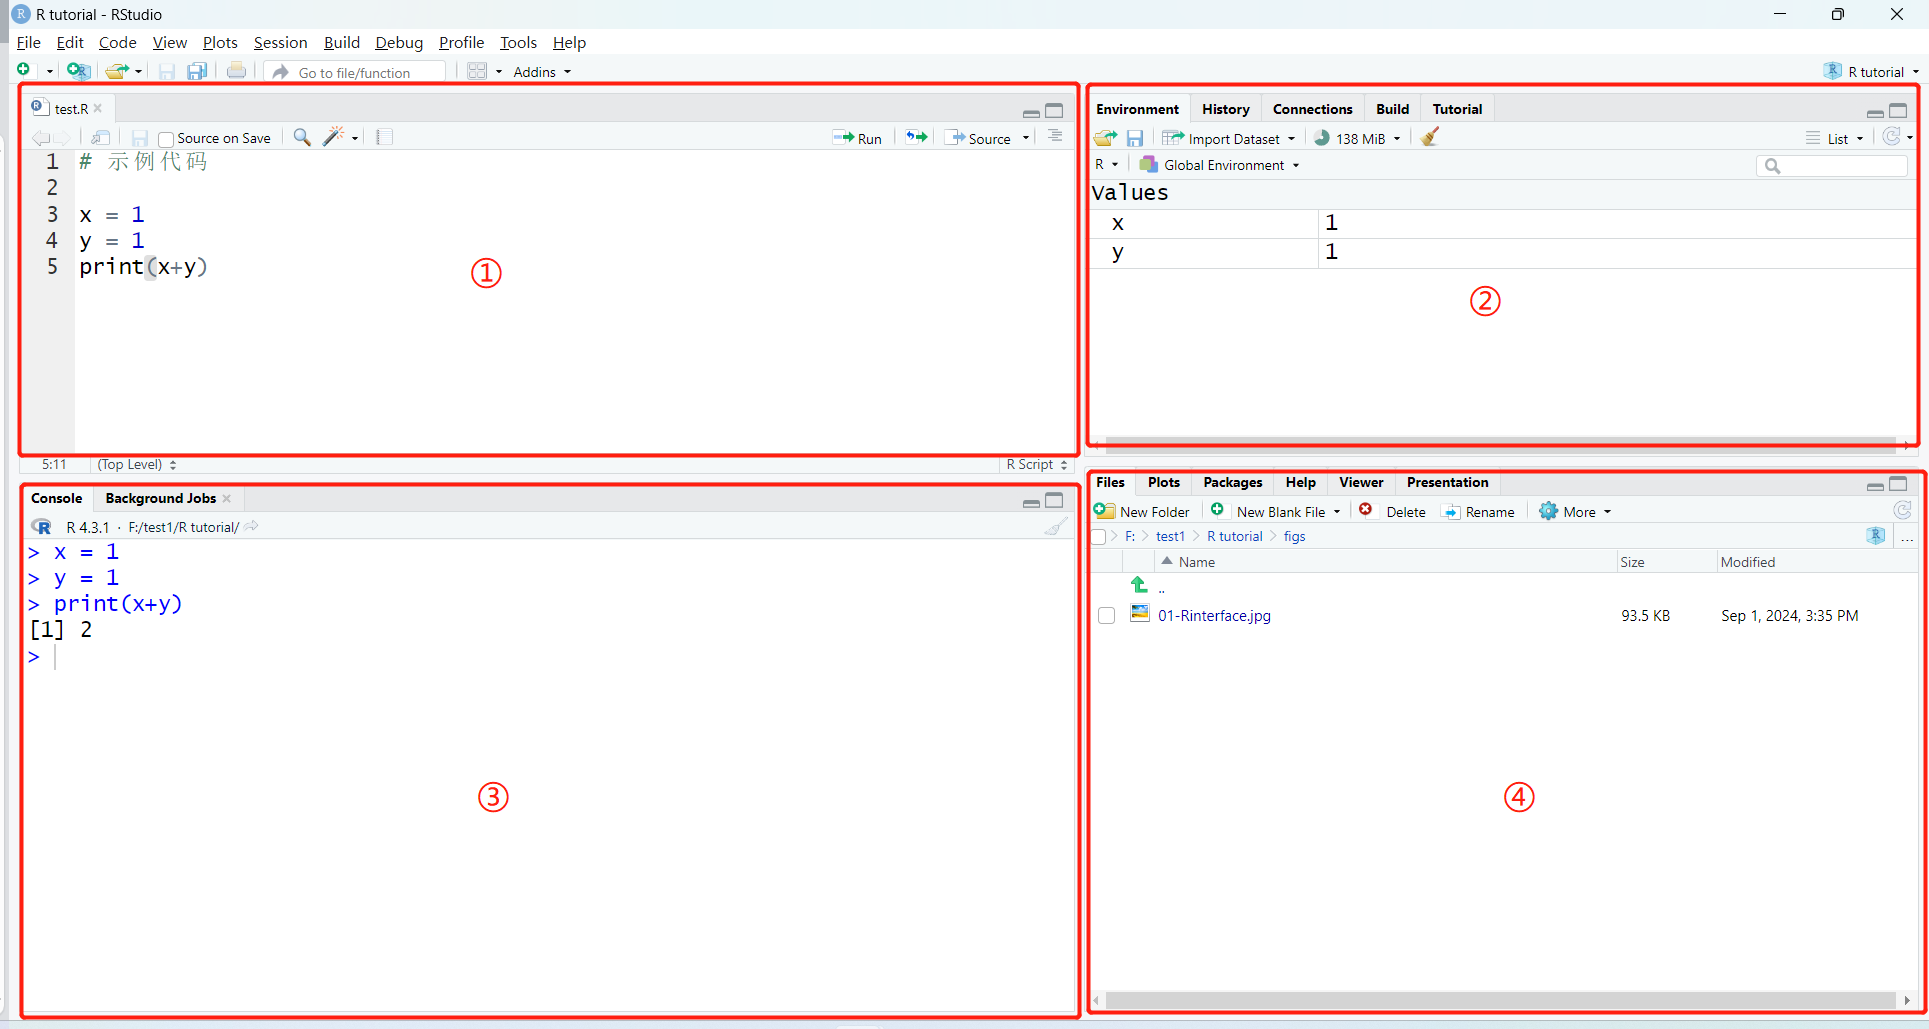
\includegraphics[width=0.8\linewidth]{figs/02-Rstudio} 

}

\caption{Rstudio软件界面}\label{fig:Rstudio}
\end{figure}

4个窗口分别是:

\begin{itemize}
\tightlist
\item
  ① 编辑器窗口:用于查看或编辑脚本,如 R 脚本等(如果未出现该窗口,用快捷键 Ctrl+Shift+N 新建一个脚本)。
\item
  ② 控制台窗口:用于输入命令,以及显示 R 脚本的执行情况。
\item
  ③ 工作区窗口:一共有4个标签页,Environment 为环境窗口,可以暂时简单理解为查看变量的窗口;History为历史窗口,用于以前运行过的命令;其他标签页暂不介绍。
\item
  ④文件等窗口:一共有6个标签页,Files 用于查看与管理文件;Plot 用于查看输出的绘图;Packages 用于管理 R 扩展包;Help 用于查看帮助文档(R 软件的文档与 RStudio 的文档都在这里)。
\end{itemize}

\subsection{控制台窗口}\label{ux63a7ux5236ux53f0ux7a97ux53e3}

开始输入一个命令,例如\texttt{co},按下 Tab 键,它会建议以 \texttt{co} 开头的函数。然后再输入\texttt{r}并选择 \texttt{cor.test} 以使用该函数。如图\ref{fig:cortest}。

\begin{figure}

{\centering 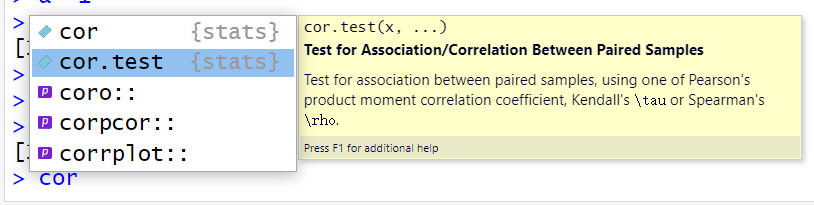
\includegraphics[width=0.8\linewidth]{figs/03-Cor.test} 

}

\caption{Tab键使用案例}\label{fig:cortest}
\end{figure}

Tab 不仅会自动补全函数和变量,还会提供函数输入参数的提示。
使用Tab键选定函数后,可以按下\textbf{F1}来获取该函数的帮助文件,按下\textbf{F2}可以显示该函数的源代码。

RStudio 中有许多实用的键盘快捷键,
比如显示快捷键菜单的快捷键是Alt + Shift + K,更多相关的内容可以参考\url{http://rstudio.org/docs/using/keyboard_shortcuts}。我们也可以在 Tools -\textgreater{} Modify Keyboard Shortcuts 中修改快捷键。

\subsection{编辑器窗口}\label{ux7f16ux8f91ux5668ux7a97ux53e3}

左上角的面板是一个编辑器,可用于编辑 R 脚本 (.R)、纯文本文件 (.txt)、HTML 网页文件、Tex 文件 (.tex) 或 RMarkdown 文件 (.rmd),后面两种文件类型可以转换为 PDF 文件。

通常我们的R代码在编辑器中完成,运行结果在控制台展示,例如可以在编辑器中输入以下代码:

\begin{Shaded}
\begin{Highlighting}[]
\NormalTok{x }\OtherTok{\textless{}{-}} \DecValTok{1}
\NormalTok{y }\OtherTok{\textless{}{-}} \DecValTok{2}
\CommentTok{\# 打印两个变量的和}
\FunctionTok{print}\NormalTok{(x}\SpecialCharTok{+}\NormalTok{y)}
\end{Highlighting}
\end{Shaded}

上述代码中,\texttt{\#} 为注释符号,后面的内容不会被当作代码执行。\texttt{\textless{}-}为R语言的赋值运算符,用于将右边的值分配(赋值)给左边的变量。在R中,也可以使用\texttt{=}来赋值,效果与\texttt{\textless{}-}相同,在大多数情况下,\texttt{=} 和 \texttt{\textless{}-} 是可以互换使用的。在R中,\texttt{\textless{}-} 更为传统且广泛使用,特别是在脚本和函数定义中,它被认为更加符合R的习惯用法。

运行上述代码有两种方式,

\begin{itemize}
\item
  选中所有代码,在编辑器左上角点击\texttt{Run},或使用快捷键Ctrl + Enter;
\item
  无需选中代码,在编辑器左上角点击\texttt{Source}。
\end{itemize}

这两种方式的主要区别是,第一种方式更加自由随意,可以运行选中的任意代码,第二种方式会直接运行整个文件中的所有代码。运行以上代码可以得到以下结果:

\begin{verbatim}
## [1] 3
\end{verbatim}

\subsection{工作区窗口}\label{ux5de5ux4f5cux533aux7a97ux53e3}

在右上角,有一个包含\texttt{Environment}和\texttt{History}选项卡的菜单。
\texttt{Environment}中列出了当前 R 会话(session)中的对象。你可以加载、保存或清除工作区中的对象。
请注意,在工作区面板下,有一个 \textbf{Import Dataset} 的选项。
\texttt{History}中列出了在控制台中输入的所有命令。你可以选择加载、保存、搜索或删除历史记录。 可以通过高亮显示一行或多行命令,并将它们发送到 \textbf{控制台}或者\textbf{编辑器},来轻松执行历史命令。
当然,在控制台也可以使用上箭头来获得历史命令。

如果我们执行了刚才编辑器中的代码,那么\texttt{Environment}会包含两个对象:\texttt{x}和\texttt{y},\texttt{History}包含了我们执行过的4行代码。

通常,我们在执行一个R程序之前会清空当前环境的中的所有变量,以避免变量污染。在R中,\texttt{rm(list\ =\ ls())} 是一个用于清除当前工作空间中所有对象的命令,其中,\texttt{ls()}函数会列出当前工作空间中所有的对象名称(变量、函数等)。

\begin{Shaded}
\begin{Highlighting}[]
\FunctionTok{ls}\NormalTok{()}
\end{Highlighting}
\end{Shaded}

\begin{verbatim}
## [1] "x" "y"
\end{verbatim}

**\texttt{rm()}函数用于删除指定的对象。由于 \texttt{ls()} 返回当前工作空间中所有对象的名称,因此 \texttt{rm(list\ =\ ls())} 的作用就是删除空间中的所有对象。

\begin{Shaded}
\begin{Highlighting}[]
\FunctionTok{rm}\NormalTok{(}\AttributeTok{list =} \FunctionTok{ls}\NormalTok{())}
\FunctionTok{ls}\NormalTok{()}
\end{Highlighting}
\end{Shaded}

\begin{verbatim}
## character(0)
\end{verbatim}

\texttt{character(0)} 表示这是一个没有任何元素的字符类型向量。

\textbf{注意}:此操作不可逆,删除的对象将无法恢复,除非你之前已经保存了它们。

\subsection{文件等窗口}\label{ux6587ux4ef6ux7b49ux7a97ux53e3}

右下角的窗口包括 \texttt{Files}, \texttt{Plots}, \texttt{Packages} 和 \texttt{Help} 等内容。

\subsubsection{Files}\label{files}

Files 是一个文件浏览器,允许你创建新文件夹、重命名文件夹或删除文件夹。点击菜单最右侧三个点的图标(\ldots)可以浏览文件夹。在\texttt{More}菜单中,你可以设置当前的工作目录(更多内容将在下文介绍)。
如果你双击一个文本文件、R文件、或html文件,它将自动在编辑器中打开。

\subsubsection{Plots}\label{plots}

Plots窗口显示在R中生成的图片,并且可以缩放、导出或删除图片。
例如,控制台窗口中输入以下命令来得到一张图片:

\begin{Shaded}
\begin{Highlighting}[]
\FunctionTok{plot}\NormalTok{(}\DecValTok{1}\SpecialCharTok{:}\DecValTok{10}\NormalTok{)}
\end{Highlighting}
\end{Shaded}

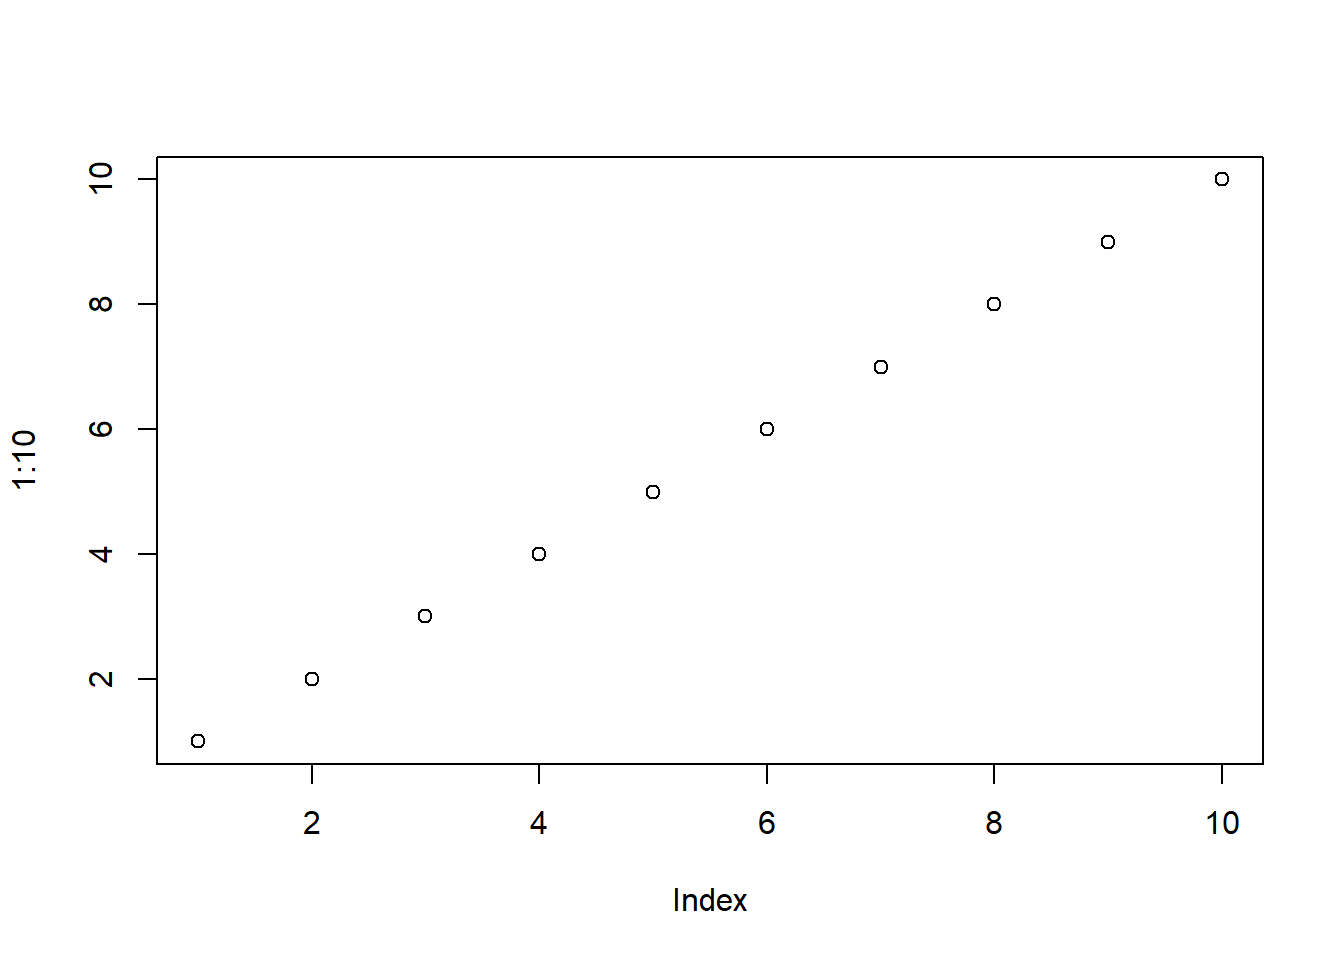
\includegraphics{_main_files/figure-latex/unnamed-chunk-7-1.pdf}

\subsubsection{Packages}\label{packages}

Packages列出了你计算机中安装的所有软件包(package)。打勾的那些软件包是当前R会话中加载的。
R包是R语言功能扩展的基本单位,它们可以包含函数、数据集、编译代码和帮助文档等。

要在R中使用一个包,首先需要安装它,然后加载它:

\begin{itemize}
\item
  \textbf{安装包}:

\begin{Shaded}
\begin{Highlighting}[]
\FunctionTok{install.packages}\NormalTok{(}\StringTok{"包名"}\NormalTok{)}
\end{Highlighting}
\end{Shaded}

  例如:

\begin{Shaded}
\begin{Highlighting}[]
\FunctionTok{install.packages}\NormalTok{(}\StringTok{"ggplot2"}\NormalTok{)}
\end{Highlighting}
\end{Shaded}
\item
  \textbf{加载包}:

\begin{Shaded}
\begin{Highlighting}[]
\FunctionTok{library}\NormalTok{(包名)}
\end{Highlighting}
\end{Shaded}

  例如:

\begin{Shaded}
\begin{Highlighting}[]
\FunctionTok{library}\NormalTok{(ggplot2)}
\end{Highlighting}
\end{Shaded}
\end{itemize}

\subsubsection{Help}\label{help}

当我们使用\texttt{?demo}时,RStudio会自动跳转到帮助界面。

在R语言中,帮助文件(help files)是用于提供关于函数、数据集或其他包内容的详细说明文档。
帮助文件的主要构成包括:

\begin{itemize}
\item
  \begin{enumerate}
  \def\labelenumi{\arabic{enumi}.}
  \tightlist
  \item
    \textbf{标题(Title)}:简要描述函数或数据集的内容。
  \end{enumerate}
\item
  \begin{enumerate}
  \def\labelenumi{\arabic{enumi}.}
  \setcounter{enumi}{1}
  \tightlist
  \item
    \textbf{描述(Description)}:对函数或数据集的简要介绍。
  \end{enumerate}
\item
  \begin{enumerate}
  \def\labelenumi{\arabic{enumi}.}
  \setcounter{enumi}{2}
  \tightlist
  \item
    \textbf{用法(Usage)}:展示函数的调用方式,包括参数列表。
  \end{enumerate}
\item
  \begin{enumerate}
  \def\labelenumi{\arabic{enumi}.}
  \setcounter{enumi}{3}
  \tightlist
  \item
    \textbf{参数(Arguments)}:详细说明函数参数的作用和含义。
  \end{enumerate}
\item
  \begin{enumerate}
  \def\labelenumi{\arabic{enumi}.}
  \setcounter{enumi}{4}
  \tightlist
  \item
    \textbf{返回值(Value)}:描述函数的输出结果。
  \end{enumerate}
\item
  \begin{enumerate}
  \def\labelenumi{\arabic{enumi}.}
  \setcounter{enumi}{5}
  \tightlist
  \item
    \textbf{示例(Examples)}:提供代码示例,演示函数的实际使用。
  \end{enumerate}
\end{itemize}

当你开始第一个 R 项目时,你需要了解如何组织 R 文件以及保存 R 脚本和输出结果。

\section{定义工作目录}\label{ux5b9aux4e49ux5de5ux4f5cux76eeux5f55}

在开始 R 编程时,首先要做的是确保能够找到你的数据,并且你的输出结果会被保存到计算机硬盘上的有用位置。因此,需要设置一个\textbf{工作目录}。

在 RStudio 中,创建一个 RStudio 项目(Project)文件夹是开始新项目的一个很好的方法,这有助于管理 R 代码、数据和结果。当然,通常的任务可以不使用项目选项,但我们仍然需要能够设置一个当前工作目录(所有输出文件都将保存在该目录中)。

有多种方式可以在 RStudio 中定义工作目录。
要更改目录:

\begin{itemize}
\item
  \begin{enumerate}
  \def\labelenumi{\arabic{enumi}.}
  \tightlist
  \item
    在 RStudio 中:\texttt{Session} \(->\) \texttt{Set\ Working\ Directory} \(->\) \texttt{Choose\ Directory};
  \end{enumerate}
\item
  \begin{enumerate}
  \def\labelenumi{\arabic{enumi}.}
  \setcounter{enumi}{1}
  \tightlist
  \item
    在 RStudio 中,点击Files标签(在右下角窗口)。使用文件浏览器窗口查看目录内容并导航到你想设置为主目录的目录。
    首先,使用文件浏览器窗口,并点击右上角的三个点图标,导航到正确的目录;然后, 当你进入正确的目录并看到你的数据文件后,点击\texttt{More}(蓝色齿轮图标),然后选择\texttt{Set\ As\ Working\ Directory}。
  \end{enumerate}
\end{itemize}

\begin{figure}

{\centering 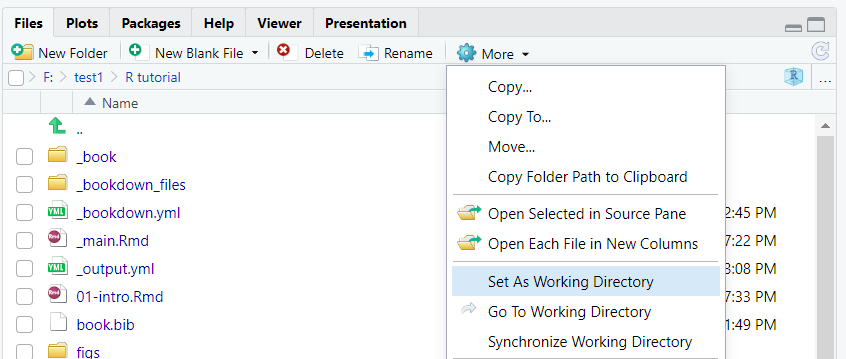
\includegraphics[width=0.8\linewidth]{figs/04-wd} 

}

\caption{查看文件并设置工作目录}\label{fig:setwd}
\end{figure}

\begin{itemize}
\item
  \begin{enumerate}
  \def\labelenumi{\arabic{enumi}.}
  \setcounter{enumi}{2}
  \tightlist
  \item
    使用打开R文件的方式启动RStudio,此时默认的工作目录就是R文件的存储路径。
  \end{enumerate}
\item
  \begin{enumerate}
  \def\labelenumi{\arabic{enumi}.}
  \setcounter{enumi}{3}
  \tightlist
  \item
    使用代码来设置工作目录。
  \end{enumerate}
\end{itemize}

\begin{Shaded}
\begin{Highlighting}[]
\CommentTok{\# 获取现在的工作目录}
\FunctionTok{getwd}\NormalTok{()}
\end{Highlighting}
\end{Shaded}

\begin{verbatim}
## [1] "F:/R_tutorial/Book/R tutorial"
\end{verbatim}

\begin{Shaded}
\begin{Highlighting}[]
\CommentTok{\# 设置工作目录}
\FunctionTok{setwd}\NormalTok{(}\StringTok{"C:/Users"}\NormalTok{)}
\FunctionTok{getwd}\NormalTok{()}
\end{Highlighting}
\end{Shaded}

\begin{verbatim}
## [1] "C:/Users"
\end{verbatim}

\textbf{特别提示}:R 中无法使用 Windows 系统中用于分隔文件路径中的文件夹的反斜杠(\texttt{\textbackslash{}})。因为在 R 中,反斜杠 是转义字符,通常用来表示特殊字符(例如 \texttt{\textbackslash{}n} 表示换行)。在下面的代码中,路径 \texttt{C:\textbackslash{}Users\textbackslash{}Rwork} 中的 \texttt{\textbackslash{}U} 被 R 解释为一个无效的转义序列,所以该代码会返回一个错误。

\begin{Shaded}
\begin{Highlighting}[]
\FunctionTok{setwd}\NormalTok{(}\StringTok{"C:\textbackslash{}Users\textbackslash{}Rwork"}\NormalTok{)}
\end{Highlighting}
\end{Shaded}

\begin{verbatim}
## Error: '\U' used without hex digits in character string (<text>:1:11)
\end{verbatim}

我们可以通过以下两种方法之一来解决这个问题:

\begin{itemize}
\tightlist
\item
  使用双反斜杠(\texttt{\textbackslash{}\textbackslash{}}):将单个反斜杠替换为双反斜杠,以告诉 R 这是一个普通的反斜杠,而不是转义字符。
\end{itemize}

\begin{Shaded}
\begin{Highlighting}[]
\FunctionTok{setwd}\NormalTok{(}\StringTok{"C:}\SpecialCharTok{\textbackslash{}\textbackslash{}}\StringTok{Users}\SpecialCharTok{\textbackslash{}\textbackslash{}}\StringTok{Rwork"}\NormalTok{)}
\end{Highlighting}
\end{Shaded}

\begin{itemize}
\tightlist
\item
  使用正斜杠(\texttt{/}):在 R 中,路径中的反斜杠可以用正斜杠 (\texttt{/}) 替代。即使在 Windows 系统上,这也是有效的。
\end{itemize}

\begin{Shaded}
\begin{Highlighting}[]
\FunctionTok{setwd}\NormalTok{(}\StringTok{"C:/Users/Rwork"}\NormalTok{)}
\end{Highlighting}
\end{Shaded}

当然感兴趣的读者也可以使用函数\texttt{file.path}来自动合成路径。

\begin{Shaded}
\begin{Highlighting}[]
\FunctionTok{file.path}\NormalTok{(}\StringTok{"C:"}\NormalTok{,}\StringTok{"Users"}\NormalTok{,}\StringTok{"Rwork"}\NormalTok{)}
\end{Highlighting}
\end{Shaded}

\begin{verbatim}
## [1] "C:/Users/Rwork"
\end{verbatim}

\subsection{使用相对路径}\label{ux4f7fux7528ux76f8ux5bf9ux8defux5f84}

在计算机文件系统中,路径(Path)是用来定位文件或文件夹的字符串。路径可以是相对的(Relative Path)或绝对的(Absolute Path)。

绝对路径是从根目录(或根文件夹)开始的完整路径,用于直接指向文件系统中的任何文件或文件夹,而不依赖于当前工作目录。它包含了从根目录到目标文件或文件夹的所有目录名,并以正确的顺序排列,中间用路径分隔符(在Windows中是,在Unix、Linux、macOS中是/)分隔。

例如,在Windows系统中,一个绝对路径可能是这样的:

\begin{Shaded}
\begin{Highlighting}[]
\ExtensionTok{C:/Users/YourName/Documents/file.txt}
\end{Highlighting}
\end{Shaded}

相对路径是相对于当前工作目录的路径。它不需要从根目录开始,而是从当前目录开始,指向目标文件或文件夹。这意味着如果你知道当前的工作目录,就可以很容易地理解相对路径。

例如,如果当前工作目录是\texttt{C:/Users/YourName/Documents},并且你想要访问同一目录下的\texttt{file.txt}文件,在运行代码时则可以直接使用以下相对路径来引用该文件:

\begin{Shaded}
\begin{Highlighting}[]
\ExtensionTok{file.txt}
\end{Highlighting}
\end{Shaded}

如果想要访问子目录Reports中的report.pdf文件,路径将是:

\begin{Shaded}
\begin{Highlighting}[]
\ExtensionTok{Reports/report.pdf}
\end{Highlighting}
\end{Shaded}

在R语言中使用相对路径是一种便捷的方式,可以避免在不同计算机或项目中由于绝对路径的差异而导致代码无法正常运行。相对路径是相对于当前工作目录(working directory)设置的路径。

以下是如何在R中使用相对路径的几个关键步骤和技巧:

\begin{itemize}
\item
  \begin{enumerate}
  \def\labelenumi{\arabic{enumi}.}
  \tightlist
  \item
    设置工作目录,工作目录是相对路径的起点。
  \end{enumerate}
\item
  \begin{enumerate}
  \def\labelenumi{\arabic{enumi}.}
  \setcounter{enumi}{1}
  \tightlist
  \item
    使用 \texttt{.} 和 \texttt{..} 进行相对路径引用
    在R中,可以使用 \texttt{.} 表示当前目录,\texttt{..} 表示上一级目录。例如:
  \end{enumerate}
\end{itemize}

\begin{Shaded}
\begin{Highlighting}[]
\CommentTok{\# 引用当前目录下的文件}
\NormalTok{data }\OtherTok{\textless{}{-}} \FunctionTok{read.csv}\NormalTok{(}\StringTok{"./data/myfile.csv"}\NormalTok{)}

\CommentTok{\# 引用上一级目录下的文件}
\NormalTok{data }\OtherTok{\textless{}{-}} \FunctionTok{read.csv}\NormalTok{(}\StringTok{"../data/myfile.csv"}\NormalTok{)}

\CommentTok{\# 引用上两级目录下的文件}
\NormalTok{data }\OtherTok{\textless{}{-}} \FunctionTok{read.csv}\NormalTok{(}\StringTok{"../../data/myfile.csv"}\NormalTok{)}
\end{Highlighting}
\end{Shaded}

在使用R完成一个项目时,通常会将项目组织成多个文件夹,如 \texttt{data/}, \texttt{scripts/}, \texttt{output/} 等。此时,相对路径在不同文件夹间访问文件就显得非常重要。

此外,使用\texttt{here} 包也可以实现管理相对路径,它会自动定位到项目的根目录,并以此为基础构建相对路径,避免了手动设置工作目录的麻烦。\texttt{here()} 函数会自动在项目的根目录下查找路径,并且无论你从哪个脚本执行代码,都可以保持路径的一致性。

\begin{Shaded}
\begin{Highlighting}[]
\CommentTok{\# 加载here包}
\FunctionTok{library}\NormalTok{(here)}

\CommentTok{\# here自动定位到工作目录,实现相对路径的效果}
\FunctionTok{here}\NormalTok{(}\StringTok{"data"}\NormalTok{, }\StringTok{"myfile.csv"}\NormalTok{)}
\end{Highlighting}
\end{Shaded}

\section{保存R对象和工作空间}\label{ux4fddux5b58rux5bf9ux8c61ux548cux5de5ux4f5cux7a7aux95f4}

在RStudio中保存变量主要涉及到将数据、模型结果或其他任何R对象保存到你的工作环境中,以便在后续的R会话(session)中能够重新访问或使用它们。然而,严格来说,``保存变量''这个术语通常指的是将变量存储在你的R会话中,以便在当前或重新加载的RStudio环境中使用。如果我们想要将变量持久化存储到文件中,以便在不同的R会话或不同的计算机上重新加载,那么需要将变量导出到文件中。

在RStudio中,当你运行一个赋值语句(如\texttt{x\ \textless{}-\ 10}),变量\texttt{x}就会被保存在当前R会话的内存中。只要不关闭RStudio或清除工作空间(Workspace),这个变量就会一直存在,并且可以在后续的代码中使用。

如果想要保存当前R会话中的变量,我们可以通过RStudio软件操作或R命令来实现。

在RStudio软件操作:找到\texttt{Session}菜单,然后选择\texttt{Save\ Workspace\ as...}来保存当前的工作空间到一个\texttt{.RData}文件。之后,我们可以通过\texttt{Load\ Workspace}来加载这个文件。

通过R命令:使用\texttt{save.image()}函数或\texttt{save()}函数。\texttt{save.image()}会保存当前工作空间中的所有变量到一个默认的文件(通常是\texttt{.RData}),而\texttt{save()}函数允许你指定要保存的变量和文件名。例如,\texttt{save(x,\ file="my\_data.RData")}会保存变量\texttt{x}到\texttt{my\_data.RData}文件中。

\begin{Shaded}
\begin{Highlighting}[]
\FunctionTok{rm}\NormalTok{(}\AttributeTok{list =} \FunctionTok{ls}\NormalTok{())                 }\CommentTok{\# 删除当前R环境中的所有对象}
\NormalTok{x }\OtherTok{\textless{}{-}} \DecValTok{10}                         \CommentTok{\# 创建一个新的数值型变量x,并将其赋值为10}
\FunctionTok{save}\NormalTok{(x, }\AttributeTok{file =} \StringTok{"my\_data.RData"}\NormalTok{) }\CommentTok{\# 保存变量x到my\_data.RData的文件中}
\FunctionTok{rm}\NormalTok{(}\AttributeTok{list =} \FunctionTok{ls}\NormalTok{())                 }\CommentTok{\# 再次删除当前R环境中的所有对象}
\NormalTok{x                               }\CommentTok{\# 这里尝试访问变量x,在实际运行时会报错}
\end{Highlighting}
\end{Shaded}

\begin{verbatim}
## Error in eval(expr, envir, enclos): object 'x' not found
\end{verbatim}

使用\texttt{load()}函数可以将\texttt{.RData}文件加载工作空间,如\texttt{load("my\_data.RData")}。

\begin{Shaded}
\begin{Highlighting}[]
\FunctionTok{load}\NormalTok{(}\StringTok{"my\_data.RData"}\NormalTok{) }\CommentTok{\# 加载之前保存的RData文件,该文件中包含了变量x }
\NormalTok{x                     }\CommentTok{\# 尝试访问变量x,访问成功}
\end{Highlighting}
\end{Shaded}

\begin{verbatim}
## [1] 10
\end{verbatim}

\section{R 包}\label{r-ux5305}

在 R 中,包是一个包含函数、数据集和其他代码的集合,用于扩展 R 的功能。R 附带了一小部分基本包,如下表:

\begin{longtable}[]{@{}ll@{}}
\toprule\noalign{}
包名 & 描述 \\
\midrule\noalign{}
\endhead
\bottomrule\noalign{}
\endlastfoot
\textbf{base} & 基本 R 函数 \\
\textbf{datasets} & 基本 R 数据集 \\
\textbf{grDevices} & 基础和网格图形的图形设备 \\
\textbf{graphics} & R 基础图形函数 \\
\textbf{methods} & R 对象的正式定义方法和类,及其他编程工具 \\
\textbf{stats} & R 统计函数 \\
\textbf{utils} & R 实用函数 \\
\end{longtable}

下面,我们将给出关于 R 包一些基本操作的介绍:

\begin{enumerate}
\def\labelenumi{\arabic{enumi}.}
\tightlist
\item
  \textbf{安装包}:
\end{enumerate}

\begin{itemize}
\item
  通过CRAN安装:CRAN(The Comprehensive R Archive Network)是R语言的主要包仓库,包含了大量的R包。在R的工作窗口或RStudio中,可以使用\texttt{install.packages()}函数来安装CRAN上的R包。例如,安装\texttt{ggplot2}包,可以使用命令\texttt{install.packages("ggplot2"})。
\item
  从本地安装:如果R包已经以压缩文件(如.tar.gz或.zip)的形式下载到本地,也可以通过RStudio的``Packages''窗口或\texttt{install.packages()}函数的\texttt{repos=NULL}参数来从本地安装。
\item
  从GitHub安装:GitHub是一个面向开源及私有软件项目的托管平台,许多开发者会在GitHub上发布自己的R包。安装GitHub上的R包需要使用\texttt{devtools}包中的\texttt{install\_github()}函数。例如,安装\texttt{rfCountData}包,对应的网址为\url{https://github.com/fpechon/rfCountData},可以使用命令\texttt{devtools::install\_github("fpechon/rfCountData")}。
\end{itemize}

\begin{enumerate}
\def\labelenumi{\arabic{enumi}.}
\setcounter{enumi}{1}
\item
  \textbf{加载包}:
  安装完R包后,需要在使用前将其加载到R的工作环境中。这可以通过\texttt{library()}函数或\texttt{require()}函数来完成。例如,加载ggplot2包,可以使用命令\texttt{library(ggplot2)}或\texttt{require(ggplot2)}。
\item
  \textbf{R包的查看}
  在R中,可以使用多种方式来查看已安装的R包及其相关信息:
\end{enumerate}

\begin{itemize}
\tightlist
\item
  使用\texttt{installed.packages()}函数可以列出所有已安装的R包及其版本信息;
\item
  使用\texttt{search()}函数可以列出当前工作环境中已加载的R包。
\item
  使用\texttt{.libPaths()}函数可以查看R包的安装路径。如果需要更改包的安装路径,可以使用\texttt{.libPaths(new="新路径")}进行设置。
\item
  使用help(package=``包名'')函数可以打开该包的帮助文档,了解包的功能和使用方法。
\end{itemize}

\begin{enumerate}
\def\labelenumi{\arabic{enumi}.}
\setcounter{enumi}{3}
\tightlist
\item
  \textbf{R包的更新和删除}
\end{enumerate}

\begin{itemize}
\tightlist
\item
  使用\texttt{update.packages()}函数来更新所有已安装的R包,或者使用\texttt{install.packages("包名",\ dependencies=TRUE)}函数来单独更新某个包及其依赖项。
\item
  使用\texttt{remove.packages("包名")}函数可以删除已安装的R包。请注意,在删除包之前,请确保不再需要该包中的任何函数或数据集。
\end{itemize}

  \bibliography{book.bib,packages.bib}

\end{document}
